% -*- mode: latex -*-

\mansection{indexing arrays, extraction, assignment}
\begin{mandesc}
   \short{indexing arrays}{various ways of indexing arrays}\\
   \short{extraction assignment deletion}{basic array operations}\\
   \short{dollar}{name the last element}\\
\end{mandesc}

\paragraph{Two ways of indexing arrays}
\begin{itemize}

\item  An array element can be adressed using its row 
 and column numbers. For example, the element in row 2
 and column 3 of the array $A$ is retrieved by
 $e = A(2,3)$ (this operation is called {\bf extraction}) 
and changed using $A(2,3) = f$ ({\bf assignment} operation). 
The row  index comes first, followed by the column index. 
Note that currently only two-dimensionnal arrays are available in nsp
(multidimensionnal array should be simulated).
The function \manlink{size}{size} is used to obtain the two dimensions
of any array.

\item A matrix $x$ with only one row is call called a {\bf row vector} 
and a matrix with only one column is called a {\bf column vector}. 
Vector elements are adressed by the preceeding way, but it is more natural
 to use a single indexing, for instance entry 3 in the
 row vector $x$ can be extracted with $e = x(1,3)$ but $e = x(3)$ works. 

\item Note that scalars and vectors are simply bidimensionnal 
arrays with special sizes, $1 \times 1$ for scalars, $1 \times n$ for
row vectors and  $m \times 1$ for columns vectors ; testing if an array
is a vector or a scalar can be done either by the size function
or directly using \manlink{isvector}{isvector} or \manlink{isscalar}{isscalar}
functions. The total number of entries in an array is obtained with
\manlink{numel}{numel} (or \manlink{length}{length} in most cases but
note a special behavior for arrays of strings).


\item An {\bf important feature} is that any matrix can be adressed with
 a single indexing (like in the fortran langage). It is  and called 
``column major order'' as illustrated by the
 following figure:    
$$
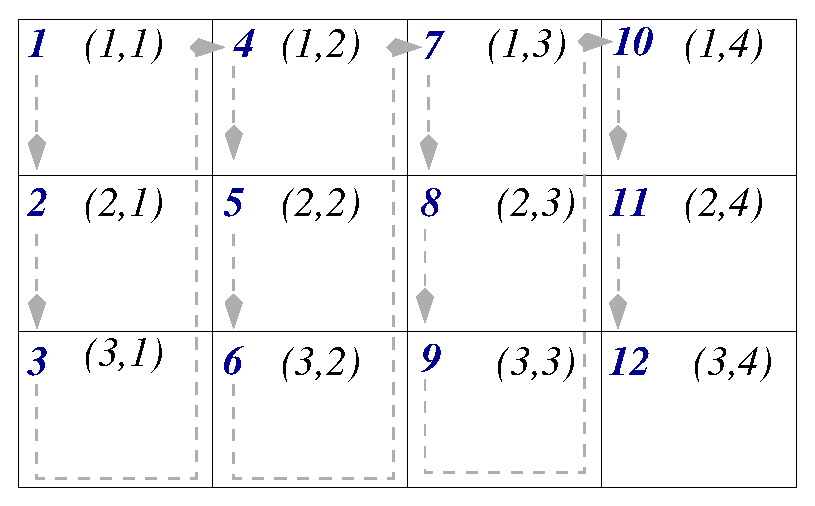
\includegraphics[width=6cm]{indexing} 
$$
The ``column major order'' (in blue) means simply that elements of the first
column are ordered first (from top to bottom) followed by those of
the second column, etc... This way of adressing array will be called
linear indexing. An exemple:
\begin{Verbatim}
A = rand(3,4)
A(2,2) = -2   // usual assignment (to the value -2) of the matrix element in position (2,2)
A(5) = 100    // assignment of the same matrix element (to the value 100) using linear indexing
\end{Verbatim}
Conversion between usual indexing and linear indexing can be done 
using the functions \manlink{sub2ind}{sub2ind}, \manlink{ind2sub}{ind2sub} (see 
also \manlink{ndind2ind}{ndind2ind}).
\end{itemize}

\paragraph{The dollar}

The dollar symbol \verb+$+ is a shortcut to denote:
\begin{itemize}
\item the last index of a vector if linear indexing is used: 
\verb+v($)+ stands for \verb+v(n)+ if the vector $v$ has $n$ elements
or for \verb+v(m*n) = v(m,n)+ if $v$ is an $m \times n$ array.
\item or the last row or column index if the ``two way'' indexing is
used: if $A$ is a $m \times n$ array then \verb+A($,3)+ stands for
\verb+A(m,3)+ and  \verb+A(2,$)+  for \verb+A(2,n)+.
\end{itemize}
Usual arithmetic operations are available with the dollar, for instance
\verb+v($-1)+ corresponds to the last but one vector element.


\paragraph{More on extraction and assignment}

\begin{itemize}
\item Another {\bf important feature} is that sub-vector or sub-matrix
      can be adressed in only one instruction for extraction or assignment:
      \begin{itemize}
      \item If $v$ is a (row or column) vector of length $n$ and  $ind$ a vector 
      of $k$ indices (also called an {\bf index vector}) 
      with values $ind(i)$ between $1$ and $n$ then:
      \begin{Verbatim}
      w = v(ind)
      \end{Verbatim}
      creates a new vector $w$ with $k$ elements such that $w(i) = v(ind(i))$, $1 \le i \le k$.
     Note that the new vector $w$ has row form if $v$ is a row vector
     and has column form otherwise (if $v$ is a column vector but also 
     if $v$ is a matrix and also when $v$ is a scalar and $ind$ an index 
     vector with all its elements equal to 1). The form of the index vector
     (row, column or even matrix) don't play any role in the form
     of $w$. Some examples:
     \begin{Verbatim}
     v = randn(1,6)
     w = v([1,3,5]) // extracts odd elements
     w = v(1:2:6)   // same thing (but with the index vector built using the a:inc:b mechanism)
     w = v(1:2:$)   // same then before but using the dollar symbol in place of its explicit value
     w = v([2,4,6]) // extract even elements
     w = v(2:2:$)   // same thing
     w = v($:-1:1)  // reverse the vector
     w = v([1,1,3,3])
     \end{Verbatim}
 
     \item If $A$ is a matrix of size $m \times n$, $indr$ an index vector of $r$ indices (with values
     between $1$ and $m$) and $indc$ an index vector of $c$ indices (with values between $1$ and $n$)
          then:
     \begin{Verbatim}
         B = A(indr,indc)
     \end{Verbatim}
     creates a new matrix $B$ of size $r \times c$ such that $B(i,j) = A(indr(i),indc(j))$, $1 \le i \le r$
     and $1 \le j \le c$. Some examples:
     \begin{Verbatim}
     A = randn(3,4)
     B = A([1,3],[1,3])
     B = A(2, :)   // extraction of the 2d row (: is a shortcut to denote all the corresponding range)
     B = A(:,3)    // extraction of the 3d column
     B = A([1,2],[4,1])
     \end{Verbatim}
 
     \end{itemize}

\item {\bf assignment} in sub-vector or sub-matrix works the same way, for instance in:
      \begin{Verbatim}
      v(ind) = w
      A(indr,indc) = B
      \end{Verbatim}
      $w$ and $B$ should have (respectively) the same matrix dimensions than what should be obtain with the extractions
      \verb+v(ind)+ and \verb+A(indr,indc)+ but some additionnal features/tricks exist:
      \begin{itemize}
      \item the rhs could be in any case a scalar, and the scalar is assigned to each matrix element denoted by the 
         indexing ;
      \item when the linear indexing is used on a matrix (which is not a vector) the rhs could be either a row
            or column vector ;
      \item the values of the indices could be larger than the matrix dimensions ; {\bf we don't recommand to use
            this rather bad trick} ; special values are used to fill the array where not defined initially 
            (0 for numerical arrays), see examples.
      \end{itemize}
     \begin{Verbatim}
     A = randn(3,4)
     A([1,2],[3,4]) = [-20,30;-30,20]  // usual assignment
     A([1,2],[3,4]) = 0  // the rhs could be a scalar
     A(2,6) = 2   // an example of assignment outside the current matrix dim => enlargement
     \end{Verbatim}
\end{itemize}

\paragraph{Indexing using boolean vectors as index vectors}  

Boolean vectors could be used instead
of numerical ones either for usual indexing or for linear indexing. The convention is simply
that true values are replaced by their corresponding index while false values are not used.
So the boolean vector \verb+[%t, %f, %f, %t, %f, %t]+ is converted as the index vector
\verb+[1, 4, 6]+. The actual usage is for expression like:
\begin{Verbatim}
     x = randn(1,8)
     x( x < 0 ) = 0  // set all negative values to zero
\end{Verbatim}
     

\paragraph{Element, row or column deletion}

Finally it is possible to delete:
\begin{itemize}
\item some elements of a vector using: \verb+x(ind) = []+
\item some rows of a matrix using:\verb+A(ind,:) = []+  
\item some columns of a matrix using:\verb+A(:,ind,:) = []+ 
\end{itemize}
Here \verb+ind+ is an index vector and all corresponding elements/rows/columns are removed.
Some examples:
\begin{Verbatim}
     x = randn(1,9)
     x(x<0) = []  // remove negative values
     A = rand(3,4)
     A(2,:) = []  // remove row 2
     A(:,[1,3]) = []  // remove column 1 and 3
\end{Verbatim}




\begin{manseealso}
    \manlink{size}{size}, \manlink{isvector}{isvector}, \manlink{isscalar}{isscalar}, \manlink{redim}{redim}, \manlink{reshape}{reshape}, \manlink{matrix}{matrix}
\end{manseealso}
